\begin{song}{title=\predtitle\centering Zatanči \\\large Jaromír Nohavica  \vspace*{-0.3cm}}  %% sem se napíše jméno songu a autor
\nejvetsi

\begin{centerjustified}

\sloka
^{Emi\z G\,}Zatanči, má milá, ^{D\z }zatanči ^{Emi\z}pro~mé oči,

^{\z G}zatanči a vetkni ^{D}nůž do mých ^{Emi}zad.

Ať tvůj ^{G}šat, má milá, ^{D}ať tvůj šat ^{Emi\z}na~zemi skončí,

ať tvůj ^{G}šat, má milá, ^{D\z}rázem je ^{Emi}sňat.

\refren
^{Emi\z G\,}Zatanči, jako se ^{D\z }okolo ^{Emi\,\,}ohně tančí,

^{\z G}zatanči jako ^{D\z }na\,\,vodě ^{Emi}loď,

^{\z G}zatanči jako to ^{D}slunce ^{Emi}mezi pomeranči,

^*{\z G}zatanči , a ^{D}pak ke mně ^{Emi}pojď.

\phantom{.}

\textbf{Mezihra}

\sloka
^{Emi\z G\,}Polož~dlaň, má milá, ^{D\z}polož dlaň ^{Emi\z}na~má prsa,

^{Emi\z G\,}polož~dlaň nestoudně ^{D}na moji ^{Emi}hruď.

^{Emi\z G\,}Obejmi, má milá, ^{D\z}obejmi ^{Emi\z}moje bedra,

^{Emi\z G}obejmi je pevně ^{D\z}a~mojí ^{Emi}buď.

\refren

\phantom{.}

\textbf{Mezihra}

\end{centerjustified}
\newpage
\begin{centerjustified}


\sloka
^{Emi\z G}Nový~den než začne, ^{D\z}má~milá, ^{Emi\z}nežli začne,

^{Emi\z G}nový~den než začne, ^{D\z}nasyť můj ^{Emi}hlad.

^{Emi\z G\,}Zatanči, má milá, ^{D}pro moje ^{Emi\z}oči~lačné,

^{Emi\z G}zatanči a já ^{D\z}budu ti ^{Emi}hrát.

\refren

\refren

\end{centerjustified}
\setcounter{Slokočet}{0}
\end{song}

\begin{figure}[h]
\predtitle\centering
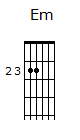
\includegraphics[width=3cm]{../Akordy/em.png}
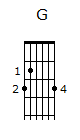
\includegraphics[width=3cm]{../Akordy/g.png}
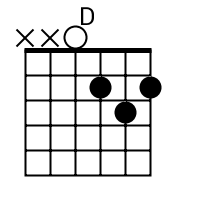
\includegraphics[width=3cm]{../Akordy/d.png}
\end{figure}
